% arara: xelatex : {options: ["-shell-escape"]}
% dokumentace k beameru: http://ftp.cvut.cz/tex-archive/macros/latex/contrib/beamer/doc/beameruserguide.pdf

% nastavení formátu prezentace 16:9 
\documentclass[czech,aspectratio=169]{beamer}

\usepackage{polyglossia}
\setmainlanguage{czech}

% nastavení vzhledu 
% další možnosti vzhledu viz https://hartwork.org/beamer-theme-matrix/
\usetheme{Madrid}
\usecolortheme{whale}

% vzhled slajdů vnitřní téma (např. vzhled odrážek)
\useinnertheme{rectangles} %možnosti: default circles rectangles rounded inmargin
% vzhled slajdů vnější téma
\useoutertheme{default} %možnosti: default, miniframes, smoothbars, sidebar, split, shadow, tree, smoothtree, infolines

% zavedeme čvutí modou barvu
\definecolor{CVUT}{HTML}{0065BD}
% čvutí modou použijeme jako hlavní barvu prezentace
\setbeamercolor{structure}{bg=white,fg=CVUT}

% jako font prezentace nadefinujeme oficiální ČVUT písmo Technika -- pokud chcete použít, musíte si font nainstalovat nebo jej nahrát na Overleaf
% https://www.cvut.cz/logo-a-graficky-manual  -- inforek, přihlášení přes celoškolské heslo
%\usepackage{fontspec}
%\setsansfont{Technika-Kniha}

% vypneme navigační panel beamer (pro zapnutí zakomentujeme)
\beamertemplatenavigationsymbolsempty

% vygenerujeme slajdy s poznámkami -- ty si můžete vytisknout a mít je na obhajobu s sebou (pokud zapomenete slova, nebo kdyby nefungovalo promítání z nějakého důvodu)
%\setbeameroption{show notes} 

% vygeneruje slajdy s poznámky vhodné pro promítání na dvou monitorech -- na obhajobu nevyužijete
%\usepackage{pgfpages}
%\setbeameroption{show notes on second screen}

% další balíčky
\usepackage{graphicx}
\usepackage{minted}
\usepackage{hyperref}
\usepackage{tikz}
\usepackage{pgfplots}
\usetikzlibrary{chains,fit,shapes}
\pgfplotsset{compat=1.15}


% Údaje o prezentaci
\title[Aplikace pro SummerJob]{Návrh a implementace aplikace pro dobrovolnickou brigádu SummerJob}
\subtitle{Diplomová práce}
\institute[FIT ČVUT v Praze]{Fakulta informačních technologií \\ České vysoké učení technické v Praze}
\author[M. Ješina]{Bc. Matyáš Ješina \\ Vedoucí práce: Ing. Marek Jílek}
\date{15. 6. 2023}
\titlegraphic{
\includegraphics[width=.1\textwidth]{logo-cvut}}


\begin{document}


  \begin{frame}
    \titlepage 
    \note{Nezapomenout pozdravit} %tohle je poznámka, ta na slajdu nebude, ale vygeneruje se vedle něj, pokud odkomentujete příkaz výše -- \setbeameroption{show notes} 
  \end{frame}
  
  % \begin{frame}
  %   \tableofcontents %generuje se automaticky z section, subsection, subsubsection
  % \end{frame}

  \section{Úvod}
  \begin{frame}{Co je SummerJob?}
    \begin{columns}
      \begin{column}{.65\textwidth}
        \begin{itemize}
          \item Letní dobrovolnická brigáda v ČR.
          \item Přibližně 150 dobrovolníků ročně.
          \item Různé typy prací.
          \item Pomoc těm, kteří na práci sami nestačí.
        \end{itemize}
      \end{column}
      \begin{column}{.3\textwidth}
        
\includegraphics[width=0.8\textwidth]{summerjob-logo}
      \end{column}
    \end{columns}
  \end{frame}
  
  \section{Cíl práce}
  \begin{frame}{Cíl práce}
    Vytvořit informační systém pro organizaci. Musí obsahovat:
    \begin{itemize}
      \item evidenci prací a účastníků,
      \item plánování prací včetně dopravy,
      \item rozhraní pro organizátory i účastníky,
      \item možnost spolupráce více organizátorů současně,
      \item tisk plánů,
      \item API pro další rozšíření.
    \end{itemize}
    Systém musí být dostupný i na mobilních zařízeních.
  \end{frame}

  \begin{frame}{Stávající řešení}
    Pro plánování byla v minulosti používána samostatná aplikace.
    \linebreak
    \linebreak
    Nevýhody:
    \begin{itemize}
      \item dostupná pouze na PC,
      \item jeden administrátorský účet,
      \item neumožňovala současnou práci více lidí,
      \item pomalé automatické plánování (50 s),
      \item nebyla dostupná pro účastníky.
    \end{itemize}
  \end{frame}

  \section{Vývoj}
  % \begin{frame}{Analýza a návrh}
  %   \begin{columns}
  %     \begin{column}{.6\textwidth}
  %       Pro tvorbu obrazu jsem zvolil TurnKey GNU/Linux, založený na distribuci Debian.
  %       \begin{itemize}
  %         \item<2-> jednoduchý na použití,
  %         \item<3-> automatizovatelný,
  %         \item<4-> bezpečný,
  %         \item<5-> rychlý,
  %         \item<6-> malý.
  %       \end{itemize}
  %     \end{column}
  %     \begin{column}{.3\textwidth}
  %       \begin{itemize}
  %         \item[]<1->{\includegraphics[width=0.8\textwidth]{turnkey}}
  %       \end{itemize}
  %     \end{column}
  %   \end{columns}
  % \end{frame}

  \begin{frame}{Analýza a návrh}
    Sběr požadavků a návrh aplikace probíhal přímo s organizátory, aby bylo zajištěno, že systém bude splňovat jejich potřeby.
    \linebreak
    \linebreak
    Základní podoba uživatelského rozhraní byla dodána před zahájením vývoje a byla dále upravována podle potřeb.
  \end{frame}

  \begin{frame}{Analýza a návrh}
    Výběr technologií:
    \begin{itemize}
      \item bezplatné použití,
      \item aktivně vyvíjené,
      \item rozšířená uživatelská základna,
      \item kvalitní dokumentace a podpora.
    \end{itemize}
  \end{frame}

  \begin{frame}{Zvolené technologie}{Webová aplikace a API}
    Pro vývoj webové aplikace byl zvolen framework Next.js.
    Klíčové vlastnosti:
    \begin{itemize}
      \item založen na React.js,
      \item umožňuje tvorbu frontendu i backendu včetně API,
      \item server-side rendering,
      \item oblíbený podle uživatelských průzkumů,
      \item aktivně vyvíjený a zdokumentovaný,
      \item využívá TypeScript.
    \end{itemize}
  \end{frame}

  \begin{frame}{Zvolené technologie}
    Dále byly využity tyto technologie:
    \begin{itemize}
      \item PostgreSQL - databáze,
      \item Prisma - ORM,
      \item Node.js - automatický plánovač,
      \item RabbitMQ - komunikace mezi službami,
      \item Docker - kontejnerizace.
    \end{itemize}
  \end{frame}

  \section{Výsledky}
  \begin{frame}{Webová aplikace}
    Výsledná aplikace je rozdělena do několika částí, které slouží ke správě:
    \begin{itemize}
      \item plánování,
      \item pracovníků,
      \item dopravních prostředků,
      \item dostupných prací,
      \item administraci.
    \end{itemize}
    
    Administrátor může organizátorům přiřazovat role pro jednotlivé části aplikace. Pracovníkům se po přihlášení zobrazí pouze detaily jejich přiřazené práce
    a mohou si ve svém profilu nastavit své osobní údaje, alergie, dostupnost atd.
  \end{frame}

  \begin{frame}{Webová aplikace}
    \begin{figure}
      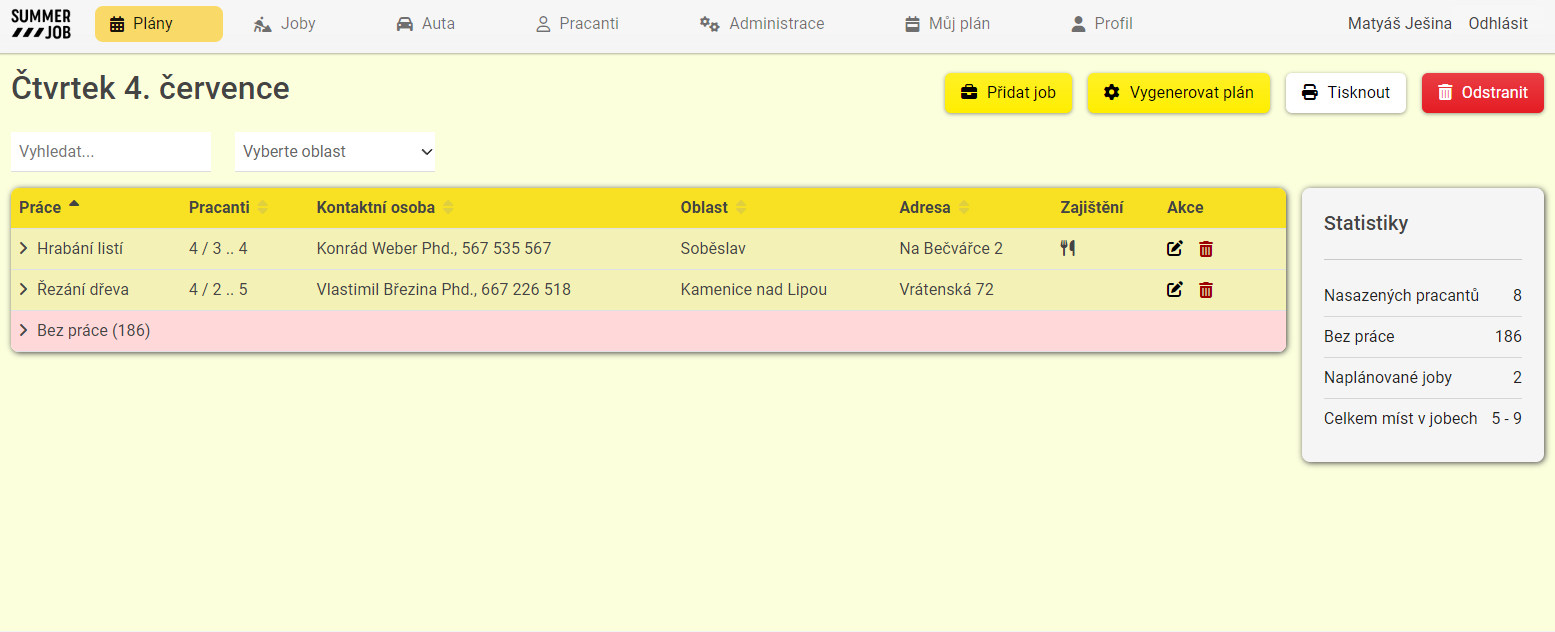
\includegraphics[width=\textwidth]{webapp}
      \caption{Webová aplikace}
    \end{figure}
  \end{frame}

  \begin{frame}{Automatický plánovač}
    Automatický plánovač je samostatná služba, která se stará o plánování prací a dopravy. Umí vytvářet plány na základě následujících kritérií:
    \begin{itemize}
      \item<2-> požadovaný počet silných a standardních pracovníků,
      \item<3-> časová dostupnost pracovníků a práce,
      \item<4-> doprava na místo (i sdílená),
      \item<5-> alergie,
      \item<6-> adorace.
    \end{itemize}
    \only<6->{Denní plán je vytvořen přibližně za 5 sekund, což představuje až desetinásobné zrychlení oproti původnímu řešení.}
  \end{frame}

  \begin{frame}{Provoz aplikace}
    Systém je od května nasazen v produkčním prostředí a bude využit během letošního ročníku akce SummerJob.
  \end{frame}

  \begin{frame}{Možnosti rozšíření}
    Všechny zdrojové kódy jsou volně dostupné. API nabízí dokumentaci pomocí nástroje Swagger (OpenAPI) a je pokryto testy.
    \linebreak
    \linebreak
    Možné rozšíření pro další ročníky:
    \begin{itemize}
      \item mobilní aplikace,
      \item pokročilý plánovač s historií a preferencemi,
      \item evidence potřebného nářadí pro práce,
      \item nástěnka s informacemi pro všechny účastníky.
    \end{itemize}
  \end{frame}

  \section{Shrnutí}
  \begin{frame}{Shrnutí}
    \begin{itemize}
      \item Cílem práce bylo vytvořit systém pro dobrovolnickou brigádu SummerJob. 
      \item Webová aplikace umožňuje evidenci prací i účastníků, práci více uživatelů současně, mobilní rozhraní i tisk plánů. 
      \item Samostatná plánovací komponenta představuje výrazné zrychlení oproti původnímu řešení.
      \item Systém je založený na moderních technologiích a je snadno rozšiřitelný.
      \item Aplikace je nasazena v produkčním prostředí a bude využita během letošního ročníku akce SummerJob.
    \end{itemize}
  \end{frame}

  \section{Otázky}
  \begin{frame}[noframenumbering]{Otázky}
    Jakou jste zvolil metodiku vývoje software a jak jste ji aplikoval? \linebreak 
    \begin{itemize}
      \item agilní vývoj,
      \item častá spolupráce a komunikace se zástupci organizace,
      \item vývoj nových funkcí na základě zpětné vazby,
      \item aplikace průběžně dostupná pro uživatele.
    \end{itemize}
   \end{frame}

   \begin{frame}[noframenumbering]{Otázky}
    Pomineme-li grafickou stránku; jakým způsobem probíhal návrh uživatelského rozhraní? \linebreak 
    \begin{itemize}
      \item základní podoba dodána před zahájením vývoje,
      \item návrh prototypů v nástroji Bootstrap Studio,
      \item průběžná konzultace s organizátory při osobních schůzkách, změny a optimalizace.
    \end{itemize}
  \end{frame}

\end{document}
